\documentclass[../TDO3.tex]{subfiles}%

\begin{document}
\section[s]"2"{Œil réduit et accommodation}
\enonce{%
	Le cristallin de l'œil est assimilable à une lentille mince de distance focale
	variable (accommodation). L'image, pour être nette, doit se former sur la rétine
	qui est située à \SI{22.3}{mm} du cristallin. Lorsque l'œil n'accommode pas
	(cristallin au repos), il voit nettement un objet situé à l'infini. Lorsqu'il
	accommode au maximum, il voit nettement un objet jusqu'à \SI{25}{cm} (valeur
	moyenne).
}%

\QR{%
	Quelles sont la vergence et la distance focale du cristallin lorsque
	l'œil voit nettement un objet placé à \SI{25}{cm}~? À l'infini~?
}{%
	~
	\smallbreak
	\vspace{-15pt}
	\begin{tcn}(data){Données}
		\begin{minipage}{0.5\linewidth}
			\begin{enumerate}
				\item Rétine = écran,
				      cristallin = lentille~;
				\item Au repos, A à l'infini~;
				\item Au \textit{proximum}, A à \SI{25}{cm}
				      ($\OA = \SI{-25}{cm}$).
			\end{enumerate}
		\end{minipage}
		\begin{minipage}{0.5\linewidth}
			\begin{center}
				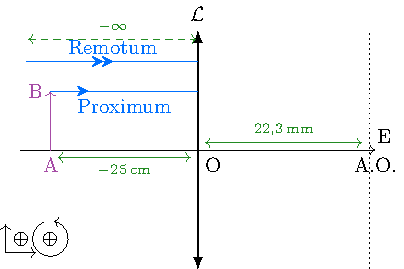
\includegraphics[width=\linewidth]{oeil_plain}
			\end{center}
		\end{minipage}
	\end{tcn}

	\begin{tcbraster}[raster columns=3, raster equal height=rows]
		\begin{tcn}(ques){Résultats attendus}
			\begin{enumerate}
				\item $\OFp _\mathrm{repos}$~?
				\item $\OFp _\mathrm{accomodation}$~?
			\end{enumerate}
		\end{tcn}
		\begin{tcn}[raster multicolumn=2](tool)'r'{Outils du cours}
			Relation de conjugaison pour une lentille mince, avec $\OAp = \obar{\rm
					OE} = \SI{22.3}{mm}$ (le principe d'un écran c'est que l'image se forme
			dessus~!!) et $\frac{1}{\OA} = 0$ quand $\OA = -\infty$
		\end{tcn}
	\end{tcbraster}

	\begin{tcn}[breakable, sidebyside](appl){Résultats}
		\[ \boxed{\OFp_\mathrm{repos} = \SI{22.3}{mm}}\]
		\begin{center}
			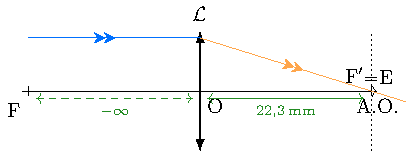
\includegraphics[width=\linewidth]{oeil_repos}
		\end{center}
		\tcblower
		\[ \boxed{\OFp_\mathrm{accomodation} = \SI{20.6}{mm}} \]
		\begin{center}
			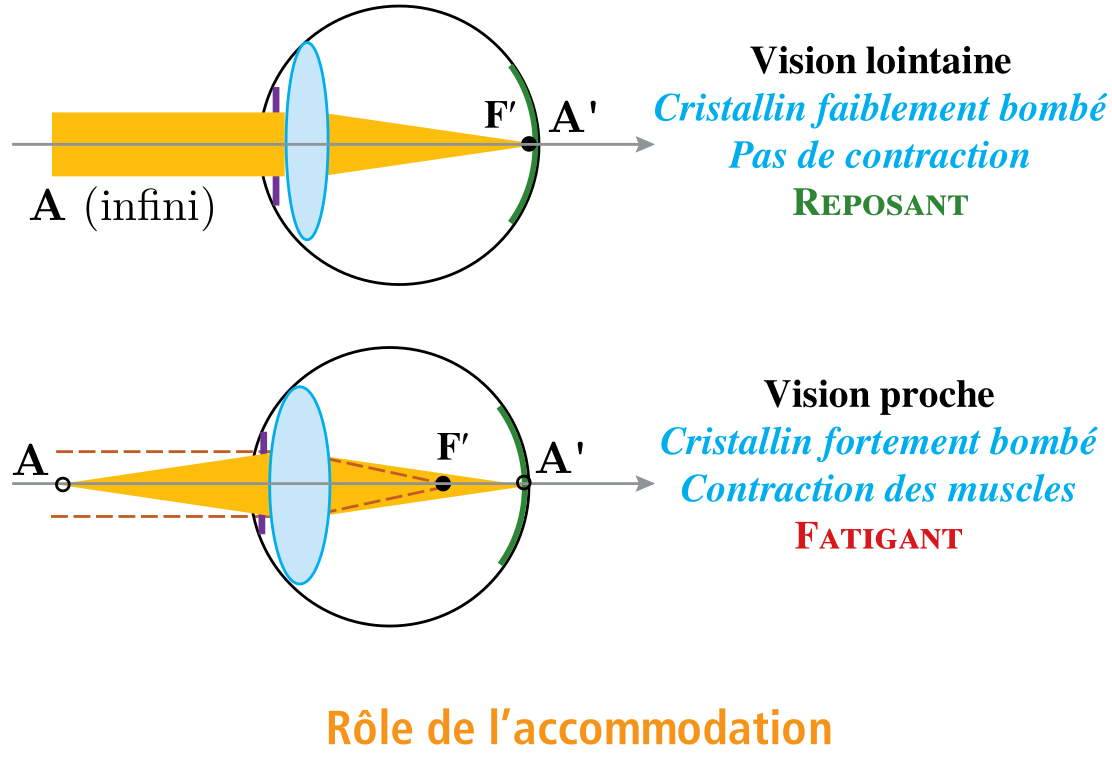
\includegraphics[width=\linewidth]{oeil_acco}
		\end{center}
	\end{tcn}
}%

\QR{%
	On observe nettement un objet de \SI{10}{cm} de haut placé à
	\SI{1.0}{m}. Quelle est la vergence du cristallin~?
}{%
  \begin{tcbraster}[raster equal height=rows, raster columns=2]
      \begin{tcn}(data){Données}
      \begin{enumerate}
        \item $\ABr = \SI{10}{cm}$
        \item $\OA = \SI{-1.0}{m}$
      \end{enumerate}
    \end{tcn}
    \begin{tcn}(tool)'r'{Outil}
      \[
        V = \frac{1}{\OAp} - \frac{1}{\OA}
      \]
    \end{tcn}
  \end{tcbraster}
	\begin{tcn}(appl){Application}
		\begin{gather*}
			\boxed{V = \frac{\OA - \OAp}{\OAp\OA}}
			\qav
			\left\{
			\begin{array}{rcl}
				\OA  & = & \SI{-1.0}{m}
				\\
				\OAp & = & \SI{22.3e-3}{m}
			\end{array}
			\right.\\
			\AN
			\xul{
				V = \SI{46}{\delta{}}
			}
		\end{gather*}
	\end{tcn}
}%

\QR{%
	Dans ces conditions d'observation, quels sont le sens et la taille de
	l'image formée sur la rétine~?
}{%
  \begin{tcbraster}[raster equal height=rows, raster columns=2]
      \begin{tcn}(ques){Résultat attendu}
      $\ABp = ?$
    \end{tcn}
    \begin{tcn}(tool)'r'{Outil}
      \[
        \frac{\ABp}{\AB} = \gamma = \frac{\OAp}{\OA}
      \]
    \end{tcn}
  \end{tcbraster}
	\begin{tcn}(appl){Application}
		\begin{gather*}
			\boxed{\ABp = \AB \times \frac{\OAp}{\OA}}
			\qav
			\left\{
			\begin{array}{rcl}
				\AB  & = & \SI{10}{cm}
				\\
				\OAp & = & \SI{2.23e-3}{m}
				\\
				\OA  & = & \SI{-1.0}{m}
			\end{array}
			\right.\\
			\AN
			\xul{
				\ABp = \SI{-0.22}{cm}
			}
		\end{gather*}
		L'image est donc renversée et rétrécie, elle fait $\SI{2.2}{mm}$. C'est
		logique en considérant la taille de la rétine de l'œil.
	\end{tcn}
}%

\end{document}
